%TEX root = ../dokumentation.tex

\chapter{Datencrawler}

\section{Vorüberlegung}
Der zu entwickelnde Datencrawler soll mit Hilfe einer IBM Connections Seedlist-\ac{URL} die vollständige Seedlist herunterladen und im \acs{JSON}-Format an eine \acs{API} senden. Dazu muss das Programm sich zunächst authentifizieren, dann den Inhalt herunterladen und sortieren und weitergeben. Danach wird nach einer Folge-\ac{URL} gesucht und dementsprechend entweder die nächste Seite der Seedlist bearbeitet oder der Timestamp abgespeichert. Zu bedenken sind dabei die Fehlerszenarien, die eintreten können. Die Authentifizierung spielt dabei eine Rolle, ebenso mögliche Fehler bei der Durchführung von einzelnen Schritten.
\begin{figure}[ht]
\centering
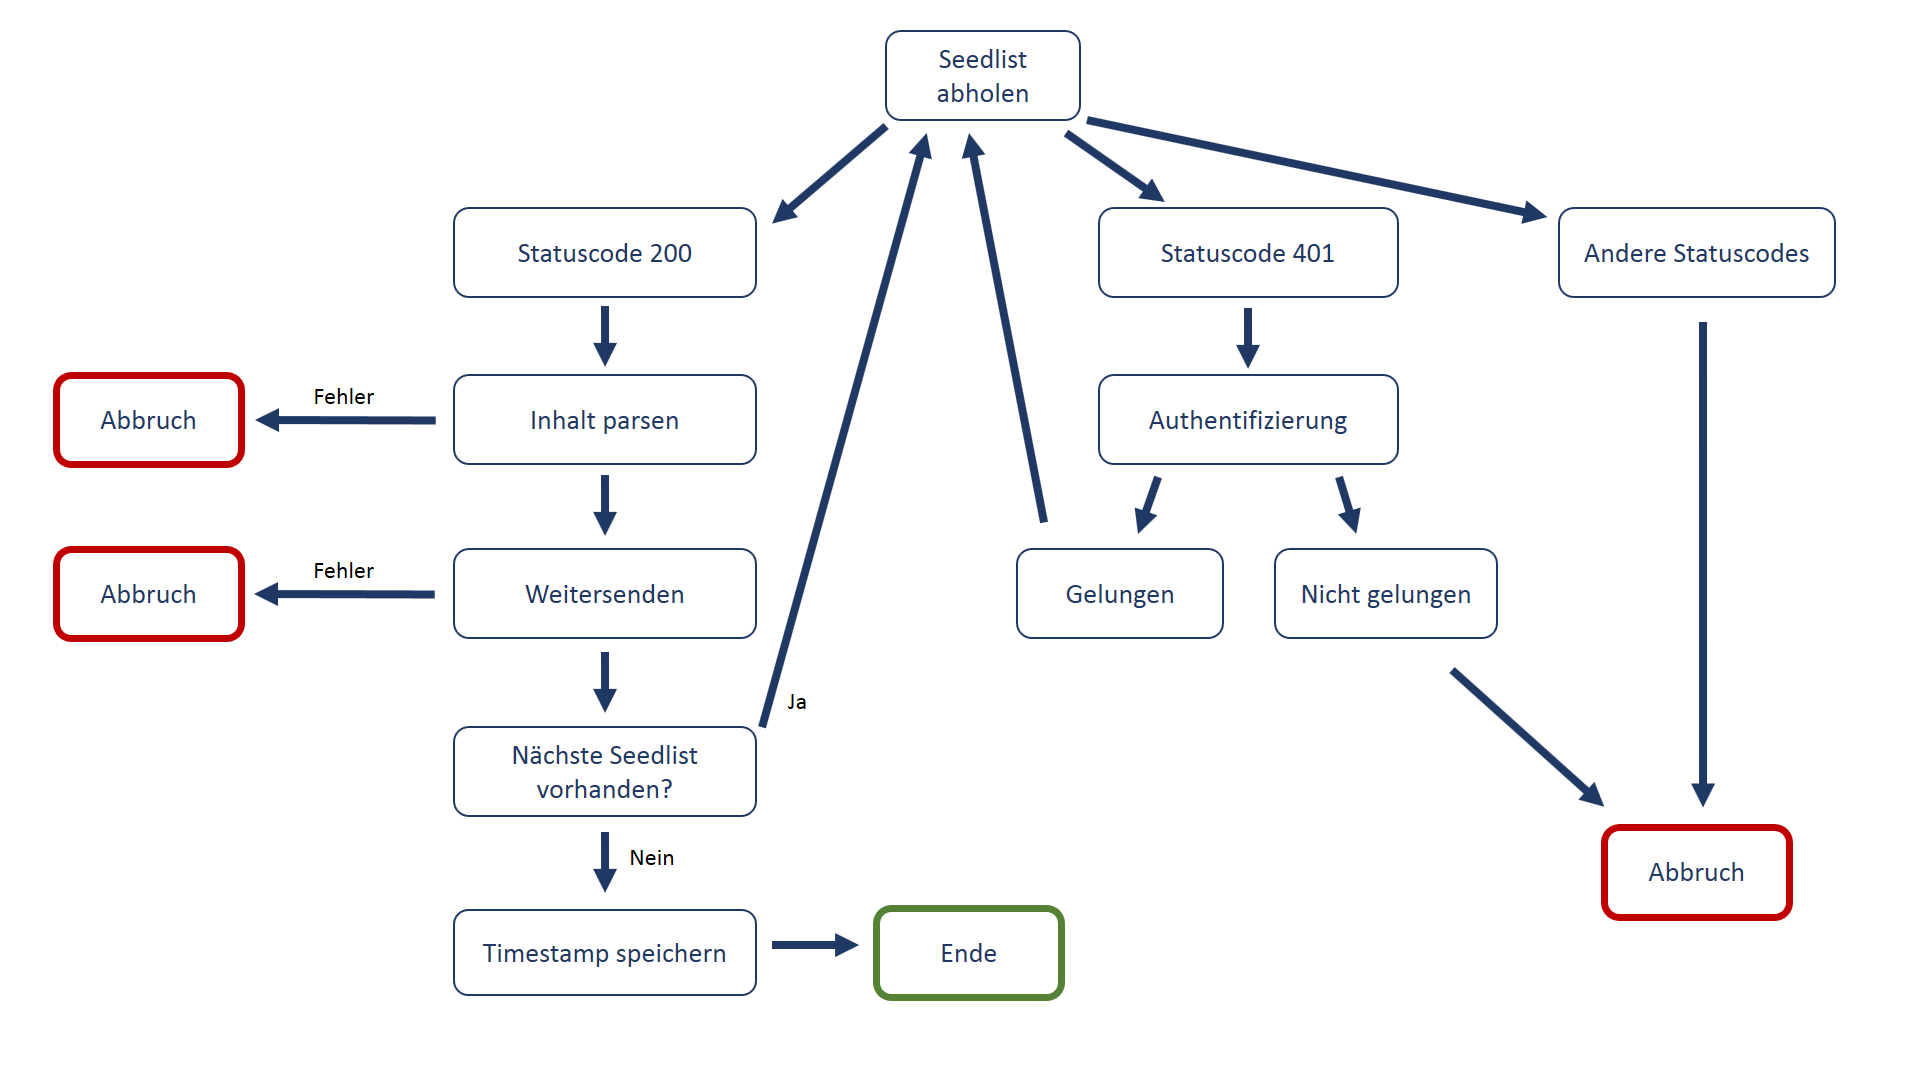
\includegraphics[width=1.0\textwidth, height=10cm]{Ablauf.png}
\caption{Ablauf des Programms}
\end{figure}

Im ersten Schritt soll der Crawler einmal versuchen, eine Seedlist abzuholen. Wenn dies nicht erfolgreich war und der HTTP-Statuscode \textit{401 Unauthorized} ist, bedeutet dies, dass das Token für die Authentifizierung abgelaufen ist oder noch keines angefordert wurde. Daher muss das Programm einen neuen Token bekommen und versucht, sich zu authentifizieren. Gelingt dies nicht, bricht es ab. Würde es erneut versuchen, sich zu authentifizieren und dies erneut fehlschlagen, würde dieser Ablauf immer wieder wiederholt werden und so eine unendliche Schleife bilden. Bei Erfolg versucht es erneut, sich die Seedlist zu holen. Sollte die Antwort bei dem Abruf der Seedlist ein anderer Statuscode als \textit{200 OK} oder \textit{401 Unauthorized} sein, hat das Programm keine weitere Möglichkeit, auf die Seedlist zuzugreifen und bricht ab.

Gelingt der Abruf, kann der Inhalt der Seedlist verarbeitet werden. Da dieser in Form von XML bereitgestellt wird, muss er zunächst geparsed werden. Danach werden die für den Expertise Locator relevanten Daten gefiltert und in ein \acs{JSON}-Format überführt. Wenn in diesem Vorgang ein Fehler auftritt, wird das Programm abgebrochen.

Der nächste Schritt ist das übergeben der Informationen an eine \acs{API}, die diese entsprechend in eine Datenbank einsortiert. Damit ist eine Seite einer Seedlist verarbeitet. Nun wird überprüft, ob es eine Folge-\ac{URL} gibt. Ist dies der Fall, beginnt der soeben beschriebene Prozess mit der entsprechenden Folge-URL von vorn. Gibt es keine Folge-\ac{URL}, existiert stattdessen ein Timestamp, der abgespeichert wird, um zukünftig beim Crawlen nicht mehr alle Informationen von der Seedlist zu bekommen, sondern nur noch die Änderungen seit diesem Timestamp.

\newpage


\section{Lösung}
\begin{sloppypar}
Der ganze Ablauf lässt sich mit zwei Funktionen umsetzen: \texttt{fetchAndProcessSeedlists} und \texttt{sendParsedResultToEE}.
\end{sloppypar}
Bereits zur Verfügung gestellt Module sind zum einen der Seedlistparser, sowie das Modul \texttt{Ltpa}, welches Methoden für die Authentifizierung bereistellt.

\textbf{fetchAndProcessSeedists:}\\
Zunächst wird ein \texttt{q}-Promise mit dem Namen \texttt{deferred} angelegt, um es später verwenden zu können. Außerdem wird ein Objekt mit dem Namen \texttt{options} angelegt, welches das Token für die Authentifizierung sowie die Seedlist-\ac{URL} enthält.
Der erste Schritt ist, die Seedlist von der vorgegebenen \ac{URL} abzuholen. Dafür wird mit dem \texttt{request}-Modul ein HTTP-Request abgesetzt.\\

\begin{lstlisting}[title=GET-Request, language=JavaScript]
response.get(options, (err, response) => {
	// verarbeiten der Antwort
}
\end{lstlisting} 

Bei dem GET-Request handelt es sich um eine asynchrone Funktion. Ihr werden die \texttt{options} und eine Callback-Funktion mitgegeben. Nun wird die Antwort auf diesen Request überprüft. Es werden hier drei Fälle unterschieden, abhängig von dem Statuscode, der in der Antwort hinterlegt ist.

Ist der Statuscode \textit{401}, bedeutet dies, dass ein Fehler bei der Authentifizierung unterlaufen ist. Im Speziellen ist dann kein gültiges Token vorhanden. Daher wird zunächst mit der \texttt{Ltpa}-Methode \texttt{getLtpaToken} ein neues Token angefordert, um damit einen neuen Versuch, auf die Seedlist zuzugreifen, zu starten. Die \texttt{getLtpaToken}-Methode ist asynchron, weshalb nachfolgende Anweisungen auf einem Promise basieren. \\

\begin{lstlisting}[title=Anfordern eines Tokens mit anschließender Weiterverwendung, language=JavaScript]
Ltpa.getLtpaToken(username, password, loginURL)
.then((newToken) => {
	return fetchAndProcessSeedlists(newToken, seedlistURL)
	.then((timestamp) => {
		deferred.resolve(timestamp);
	})
	.fail((error) => {
		deferred.reject(error);
	});
})	
.fail((error) => {
	deferred.reject(error);
});
\end{lstlisting}

Sobald ein neues Token zur Verfügung steht, wird die \texttt{fetchAndProcessSeedlists}-Funktion rekursiv mit dem neuen Token aufgerufen (Zeile 3). Ist dies abgeschlossen, wird das Promise durch \texttt{deferred.resolve} nach dem Timestamp aufgelöst (Zeile 5). Schlägt jedoch entweder das Anfordern eines neuen Tokens oder das Abholen der Seedlist fehl, so wird das Promise abgelehnt mit \texttt{deferred.reject} (Zeilen 7 bis 12).

Ist bei dem Aufruf der \texttt{fetchAndProcessSeedlists}-Funktion der Statuscode \textit{200}, so kann nun auf den Inhalt der Seedlist zugegriffen werden. Dieser wird zunächst decodiert und dann geparsed. Der Vorgang des Parsens ist wieder asynchron, weshalb erneut Promises zum Einsatz kommen. \\

\begin{lstlisting}[title=Verwendung von Promises, language=JavaScript]
seedlistParser.parse(seedlist)
.then((parsedResult) => {
	handler.sendParsedResultToEE(parsedResult);
});
\end{lstlisting}

\begin{sloppypar}
Dieser Code führt, sobald das Parsing abgeschlossen ist, die \texttt{sendParsedResultToEE}-Funktion aus. Damit ist eine Seite der Seedlist abgearbeitet. Danach wird überprüft, ob es noch weitere Seiten gibt. Auch dies geschieht mit Hilfe eines Promises im Anschluss an den soeben gezeigten Code. \\
\end{sloppypar}

\begin{lstlisting}[title=Suche nach einer weiteren Seedlist-URL, language=JavaScript]
.then((parsedResult) => {
	if (parsedResult && parsedResult.headers && parsedResult.headers.nextPage) {
		return fetchAndProcessSeedlists(token, parsedResult.headers.nextPage)
	}
});
\end{lstlisting}

Das Ergebnis nach dem Parsen ist kein \ac{XML} mehr, sondern ein Objekt im \acs{JSON}-Format, sodass auf die nächste Seedlist-\ac{URL} einfach mit \texttt{parsedResult.headers.nextPage} zugegriffen werden kann. Mit dieser neuen \ac{URL} wird dann erneut die \texttt{fetchAndProcessSeedlists}-Funktion aufgerufen. Da diese dann durch alle Seedlist-Seiten iteriert, wird nach dem rekursivem Aufruf das Promise in den \textit{fulfilled}-Zustand versetzt und wieder mit \texttt{resolve} nach dem Timestamp aufgelöst. Gibt es jedoch keine weitere Seedlist-\ac{URL}, so wird das Promise direkt nach dem Timestamp aufgelöst. Auch hier wird bei einem Fehler bei dem erneuten Aufruf von \texttt{fetchAndProcessSeedlists} mit \texttt{deferred.reject} der Fehler abgefangen.

Der dritte Fall, der in dieser Funktion auftreten kann, ist ein Statuscode, der weder \textit{200} noch \textit{401} ist. In diesem Fall wird das Promise sofort mit \texttt{deferred.reject} abgelehnt, da ein anderer Statuscode auf enen Fehler hinweist, auf den das Programm keinen Einfluss hat. Daher wird es in diesem Fall abgebrochen.

Nachdem die Seedlist erfolgreich geparsed werden konnte, wird die Funktion \texttt{sendParsedResultToEE} aufgerufen. Diese Funktion ist für die richtige Formatierung des Inhalts verantwortlich. Direkt nach dem Parsen sind in dem \ac{JSON}-Dokument noch einige Informationen enthalten, die für die \acl{EE} irrelevant sind, wie zum Beispiel Folge-\acp{URL} oder eine AtomAPISource. Daher müssen die relevanten Daten herausgefiltert und in eine verwertbare Struktur gebracht werden.Um den Code zu verkürzen und zu vereinfachen, wird dafür das Node-Modul \texttt{lodash} verwendet. Die dazugehörige Variable ist ein Unterstrich.

Die Funktion \texttt{sendParsedResultToEE} ist unterschiedlich, abhängig von der Seedlist. Beispielsweise wird bei der Seedlist von Blogs nach Blogs, Blogeinträgen und Kommentaren unterschieden. Bei den Communities hingegen werden Communities und Bookmarks erfasst. Der Mechanismus wird hier anhand der Blogs-Komponente erläutert.

Für die Blogs-Komponente werden je ein Array für Blogs, Blogeinträge und Kommentare angelegt. In dem \acs{JSON}-Dokument sind die Informationen nach dem Parsen in einem Array von Einträgen arrangiert. Mit der \texttt{lodash}-Funktion \texttt{forEach} kann durch das ganze Array iteriert werden. Bei jedem Eintrag wird überprüft, ob er bestimmte Werte hat, die ihn als ein bestimmtes Element auszeichnen. Ein Blog hat das Attribut \texttt{type} mit dem dazugehörigen Wert \texttt{application/blog}. Außerdem hat er die Attribute \texttt{title} und \texttt{details}. Bei einem Blogeintrag ist der \texttt{type} gleichgesetzt mit \texttt{blogs/entry}. Auch hier gibt es die Attribute \texttt{title} und \texttt{details}. Ein Blogeintrag kann außerdem Kommentare haben, die in sich in einem weiteren Array strukturiert sind. 

Wenn die Art des Eintrags in der Seedlist festgestellt ist, müssen die Informationen neu angeordnet werden. Da jede Art von Eintrag einen eigenen Array hat, werden die Daten mit der \texttt{push}-Methode in den Array eingefügt. \\

\begin{lstlisting}[title=Struktur von Informationen über einen Blog, language=JavaScript]
blogs.push({
	users: [ { uid: value.uid, }, ],
	id: value.id,
	title: value.title,
	summary: value.details,
	tags: value.tags || [],
});
\end{lstlisting}

Zuerst wird hier der Nutzer mit einer ID angegeben. Die Nutzer werden hier in einem Array dargestellt, da diese Struktur kompatibel zu anderen Informationsquellen, von denen andere IDs für den gleichen Nutzer kommen können, sein soll. Daher werden hier die Vorbereitungen dafür getroffen. Weiterhin relevant sind die ID des Blogs, der Titel, die Zusammenfassung und die Tags, mit denen der Blog versehen wurde. Diese Eigenschaften enthalten Schlagworte, die für die Identifikation eines Experten Hinweise liefern. Einige Blogs haben bisher keine Tags erhalten, weshalb in diesem Fall, für die Tags nur ein leeres Array hinzugefügt wird.

Ähnlich verhält es sich mit Blogeinträgen: \\

\begin{lstlisting}[title=Struktur von Informationen über einen Blogeintrag, language=JavaScript]
blogEntries.push({
	id: value.id,
	users: [
		{
			uid: value.uid,
		},
	],
	title: value.title,
	content: striptags(value.details),
	tags: value.tags || [],
});
\end{lstlisting}

Auch hier werden die Nutzer in einem Array gespeichert und die ID des Eintrags, der Titel, der Inhalt und die Tags festgehalten. Der Inhalt wird dabei vorher noch mit der \texttt{striptags}-Funktion bearbeitet, da dieser in \ac{HTML}-Format vorliegt und die \ac{HTML}-Tags entfernt werden müssen.

Zuletzt werden außerdem die Kommentare in dem entsprechenden Array dargestellt. \\

\noindent
\begin{minipage}{\linewidth}
\begin{lstlisting}[title=Struktur von Informationen über einen Kommentar, language=JavaScript]
entryComments.push({
	id: comment.id,
	users: [
		{
			uid: comment.uid,
		},
	],
	content: comment.blogCommentDetails,
});
\end{lstlisting}
\end{minipage}

Die Nutzer werden wieder in einem Array dargestellt und es wird sowohl eine ID als auch der tatsächliche Inhalt des Kommentar abgespeichert.

